\section{Introducing \acs{NMR}}

\subsection{A Brief History of NMR}
The origins of \ac{NMR} can be traced back to 1945, when independent work by
Felix Bloch on water\cite{Bloch1946} and Edward Purcell on
parrafin\cite{Purcell1946} gave rise to the first illustrations of nuclear
magnetic resonances in condensed phases. The two hadn't met before their
respective papers were published with about a month's
separation\cite{Becker1993}. Both received the Nobel Prize in Physics in 1952
for their pioneering work in the field. A notable mention should also be given
to Yevgeny Zavoisky, the father of Electron Paramagnetic Resonance, who
probably observed NMR as far back as 1941\cite{Eaton1998}. Alas, he dismissed
his results as irreproducible. In 1949 and 1950, work investigating \ac{NMR}
spectra from compounds containing Cu, \textsuperscript{31}P,
\textsuperscript{14}N, and \textsuperscript{19}F nuclei illustrated the concept
of the chemical shift\cite{Knight1949, Proctor1950, Dickinson1950}, in which
nuclei in different chemical environments exhibit non-identical resonant
frequencies.  Chemists regarded these results with great interest, as these
findings suggested that \ac{NMR} could give insights into molecular structure.

Russel Varian secured the first patent for a commercial \ac{NMR} machine, with
a \qty{30}{\mega\hertz} spectrometer following soon after. The first
spectrometers functioned by slowly sweeping the magnetic field,
causing spins to come into resonance at different times, in a process referred
to a continuous wave spectroscopy. Richard Ernst and
Weston Anderson, working at Varian Inc. at the time, proposed an alternative
method: pulsed \ac{FT} spectroscopy\cite{Ernst1966}. This was not seen as a
fruitful endeavour by the company, largely because of the very long time it
took to digitise the signal, and subsequently compute its FT\cite{Freeman2015}.
Instead, the first commercial pulsed \ac{FT} spectrometer was produced by
Bruker Corp. in 1969, which revolutionised NMR. The emergence of the
Cooley-Tukey's \ac{FFT} algorithm\cite{Cooley1965} led to vast improvements in
the speed with which experiments could be conducted, which incentivised the
development of the new \ac{FT} approach.

The idea of 2D NMR spectroscopy was proposed by Jean Jeener in
1971\cite{Jeener1971, Jeener2016}, which Ernst and co-workers showcased a few
years later in the form of a \acs{COSY} experiment\cite{Aue1976a}. The use of
multiple dimensions to spread out signals enabled vastly more complex
structures to be studies. In 1985, a report of the first protein assigned by
\ac{NMR} (using \acs{COSY} and \acs{NOESY}) was presented by Kurt W\"utrich and
co-workers\cite{Williamson1985}. Over time, extensive developments in
techniques for biomolecular systems have occurred, including the creation of 3D
and 4D experiments\cite{Marion1989, Kay1990}, as well \acs{TROSY}
experiments\cite{Pervushin1997} for the study of large proteins.

\ac{NMR}'s significance as an analytical tool is evidenced by Nobel Prizes in
Chemistry being awarded for work in the field on two separate occasions. First,
Ernst received the prize in 1991 ``for his contributions to the development of
the methodology of high resolution \acl{NMR}"\cite{Ernst1992}. In 2002,
W\"uthrich was recognised ``for his development of \acl{NMR} for determining
the three-dimensional structure of biological macromolecules in
solution"\cite{Wuthrich2003}.

\subsection{Nuclear Spin and Magnetism}

\ac{NMR} relies on \textit{spin}, an intrinsic property of certain nuclei
(along with other elementary particles) which, along with orbital angular
momentum, is one of the two sources of angular momentum in quantum mechanics.
The angular momentum associated with a nuclear spin is characterised by the
quantum number $I$, which may be integer or half-integer. Spin-\nicefrac{1}{2}
nuclei are the most commonly studied in \ac{NMR}, as those with $I >
\nicefrac{1}{2}$ often have very short-lived excited states, due to electric
quadrupole effects. A rigorous description of \ac{NMR} requires quantum
mechanics, with many excellent texts devoted to the
subject\cite{Abragam1961,Goldman1988,Cavanagh2007}. However, a basic
appreciation can be gained using the Bloch model, a semi-classical description
of the simplest of system to study: a ensemble of spin-$\nicefrac{1}{2}$
nuclei.

The nuclear spin angular momentum $\symbf{I} \in
\mathbb{R}^3$ is a vector with (square) magnitude:
\begin{equation}
  \symbf{I}^2 = \symbf{I} \cdot \symbf{I} = \hbar I (I + 1),
  \label{eq:I-squared}
\end{equation}
where $\hbar = \nicefrac{h}{2 \pi}$ is the reduced Planck constant. While it
is not possible to specify multiple components of the angular momentum
simultaneously due to the uncertainty principle, it is possible to specify one
of these, along with $\symbf{I}^2$. Conventionally, this is chosen to be the
z-component, for which
\begin{equation}
  I_z = \hbar m,
  \label{eq:Iz}
\end{equation}
with $m \in \lbrace -I, -I+1, \cdots, +I \rbrace$. \eqref{eq:I-squared} \& \eqref{eq:Iz}
imply that the orientation of the z-component may only adopt certain discrete
values (i.e. it is quantised). A nucleus with non-zero spin has an associated
\textit{magnetic moment}, given by:
\begin{equation}
  \symbf{\mu} = \gamma \symbf{I} \implies \mu_z = \gamma I_z = \gamma \hbar m.
\end{equation}
$\gamma$ is a proportionality constant called the \textit{gyromagnetic ratio},
which is dependent on the nucleus of interest. Table \ref{tab:nuclei} provides
the gyromagnetic ratios for a few nuclei commonly encountered in NMR, along
with a few which alas are spin-$0$.

\setlength\extrarowheight{3pt}
\begin{table}
    \begin{center}
        \begin{tabular}{ c c c c }
            \toprule
            Nucleus & $I$ & $\gamma (\si{\radian \per \tesla \per \second})$ & Relative Abundance (\%) \\
            \midrule
            \textsuperscript{1}H & \nicefrac{1}{2} & \num{2.6752e8} & 99.9885 \\
            \textsuperscript{2}H & 1 & \num{4.1066e7} & 0.0115 \\
            \textsuperscript{6}Li & 1 & \num{3.9371e7} & 7.59 \\
            \textsuperscript{7}Li & \nicefrac{3}{2} & \num{1.0398e8} & 92.41 \\
            \textsuperscript{12}C & 0 & - & 98.93 \\
            \textsuperscript{13}C & \nicefrac{1}{2} & \num{6.7283e7} & 1.07 \\
            \textsuperscript{14}N & 1 & \num{1.9338e7} & 99.636 \\
            \textsuperscript{15}N & \nicefrac{1}{2} & \num{-2.7126e7} & 0.364 \\
            \textsuperscript{16}O & 0 & - & 99.756 \\
            \textsuperscript{17}O & \nicefrac{5}{2} & \num{-3.6281e7} & 0.038 \\
            \textsuperscript{19}F & \nicefrac{1}{2} & \num{2.5162e8} & 100 \\
            \textsuperscript{31}P & \nicefrac{1}{2} & \num{1.0839e8} & 100 \\
            \bottomrule
        \end{tabular}
    \end{center}
    \caption{
        A table of regularly encountered nuclei in \acs{NMR}, along with common
        nuclei which are not \acs{NMR} active.
    }
    \label{tab:nuclei}
\end{table}

Without the presence of an external magnetic field, the nuclear spin states of
different $m$ are degenerate. However, when subjected to such a field, the
\emph{Zeeman effect} is observed, in which the relative energies of the
different states diverge. The associated energy of a given magnetic moment is
given by
\begin{equation}
  E = - \symbf{\mu} \cdot \symbf{B}_0
\end{equation}
where $\symbf{B}_0 \in \mathbb{R}^3$ is the magnetic field vector. It is
conventional to define the external field as directed along the laboratory
$z$-axis, such that $B_{0,x} = B_{0,y} = 0$ and $B_{0,z} = B_0$ where $B_0$ is
the magnetic field strength. The energies of the individual spin states are
therefore
\begin{equation}
  E_m = - \gamma I_z B_0 = -m \hbar \gamma B_0
\end{equation}
Figure \ref{fig:energy_levels} illustrates how the relative energies of different
spin states vary with $B_0$.

\begin{figure}
    \centering
    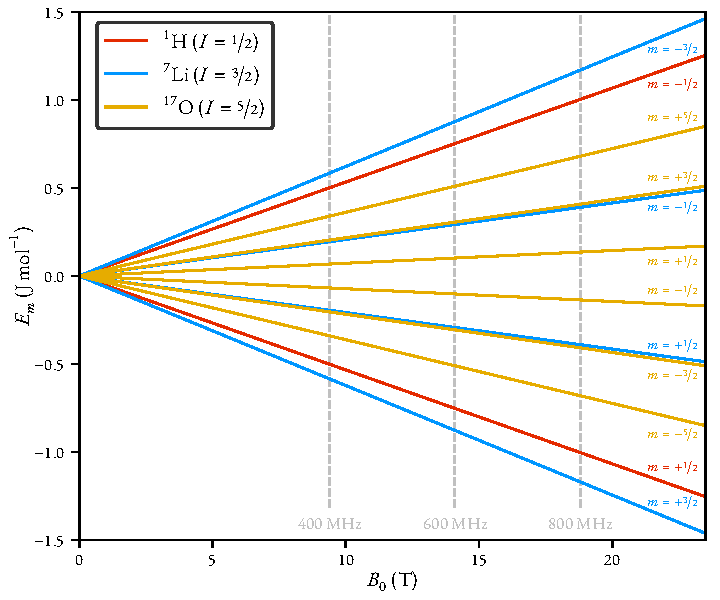
\includegraphics{energy_levels/energy_levels.pdf}
    \caption[
        The variation of energy of the spin states of \proton,
        \textsuperscript{7}Li, and \textsuperscript{17}O with external magnetic
        field strength.
    ]{
        The variation of energy of the spin states of \proton,
        \textsuperscript{7}Li, and \textsuperscript{17}O with external magnetic
        field strength ($B_0$), up to \qty{23.5}{\tesla}, which is
        approximately the strength of a \qty{1}{\giga \hertz} \ac{NMR} magnet.
        Three common field strengths for commercial NMR magnets are indicated:
        \qty{9.40}{\tesla} (\qty{400}{\mega\hertz}), \qty{14.10}{\tesla}
        (\qty{600}{\mega\hertz}), and \qty{18.79}{\tesla}
        (\qty{800}{\mega\hertz}).
    }
    \label{fig:energy_levels}
\end{figure}

\ac{NMR} samples comprise a vast ensemble of equivalent spin systems, and it is
the macroscopic properties of the sample that are observed.
At thermal equilibrium, the various spin states will be disproportionately
populated in accordance with the Boltzmann distribution, with lower energy
states being more heavily populated. For example, an ensemble of
non-interacting spin-$\nicefrac{1}{2}$ nuclei with $\gamma > 0$ will have a
more populated $m = +\nicefrac{1}{2}$ (\textalpha) state, relative
to the $m = -\nicefrac{1}{2}$ (\textbeta) state. Due to the very small relative
energy difference however, it should be noted that the discrepancy in state
populations is very small.
The ensemble acquires a net (bulk) magnetic moment $\symbf{M}$, given by the
summation of all the individual spin moments:
\begin{equation}
    \symbf{M} = \sum\limits_{n=1}^{N} \symbf{\mu}_n,
\end{equation}
where $N \gg 1$ is the number of spins in the ensemble.
At equilibrium, the $x$- and $y$-components of the bulk magnetisation are zero,
i.e.
\begin{equation}
    \sum_{n=1}^{N} \mu_{x,n} = \sum_{n=1}^{N} \mu_{y,n} = 0,
\end{equation}
such that the bulk magnetisation is collinear with the field direction, with a
magnitude $M_0$, which is approximately given by
\begin{equation}
    M_0 \approx \frac{N \gamma^2 \hbar^2 B_0 I (I + 1)}{3 k_{\text{B}} T},
\end{equation}
where $k_{\text{B}}$ is the Boltzmann constant, and $T$ is the sample
temperature. For purposes of experiment sensitivity, it is hence desirable to
utilise nuclei with (a) high natural abundance (which affects $N$) and high
gyromagnetic ratio. Along with other favourable attributes such as its ubiquity
in organic molecules, \proton\ is therefore by far the most popular nucleus to
study using \ac{NMR}.

In the presence of a magnetic field, the bulk magnetism experiences a torque,
with its of rate of change with respect to time being
\begin{equation}
  \frac{\mathrm{d}\symbf{M}(t)}{\mathrm{d}t} = \symbf{M}(t) \times \gamma \symbf{B}(t).
  \label{eq:M-cross-B}
\end{equation}
The essence of \ac{NMR} is to manipulate and subsequently detect the evolution
of $\symbf{M}$. Manipulation is achieved by applying short bursts of \ac{RF}
radiation known as \emph{pulses} which perturb the net magnetic field from
$\symbf{B}_0$. The contribution to the field induced by pulses is commonly
denoted $\symbf{B}_1(t)$, such that at any given time
\begin{equation}
    \symbf{B}(t) = \symbf{B}_0 + \symbf{B}_1(t).
\end{equation}
Whenever the magnetisation vector is not collinear with the field vector\footnote{
    The cross product of two collinear vectors is $0$, so $\symbf{M}$ remains
    fixed when it is aligned with $\symbf{B}$, as is the case at equilibrium.
}, it
undergoes \emph{precession} about the field vector. Free precession occurs
when the magnetisation is aligned away from the $z$-axis, and $\symbf{B}_1 =
\symbf{0}$, such that
\begin{equation}
  \frac{\mathrm{d}\symbf{M}(t)}{\mathrm{d}t} =
  -\gamma B_0
  \begin{bmatrix}
      M_y & -M_x & 0
  \end{bmatrix}^{\mathrm{T}},
\end{equation}
i.e. the magnetisation precesses around the $z$-axis at the \emph{Larmor
frequency} $\omega_0 = -\gamma B_0$.\footnote{
    While the SI base unit of magnetic field strength is the Tesla
    (\unit{\tesla}), when referring to the field strength that a spectrometer
    operates at, it is common to use \unit{\mega\hertz} instead. This refers to
    the (negative) Larmor frequency of an isolated \proton\ nucleus at the
    given field strength. For example, a \qty{500}{\mega\hertz} spectrometer
    operates at a field strength of
    $\nicefrac{\qty{5e8}{\hertz}}{\qty{4.2577e7}{\per\tesla\hertz}}
    \approx \qty{11.74}{\tesla}$.
}

Assuming the \ac{RF} field is linearly polarised along the $x$-axis, it can be
written to a high degree of accuracy as
\begin{equation}
    \symbf{B}_1(t) = B_1\left(
        \cos(\omega_{\text{RF}} t + \phi_{\text{RF}}) \symbf{i} +
        \sin(\omega_{\text{RF}} t + \phi_{\text{RF}}) \symbf{j}
    \right),
\end{equation}
with $\symbf{i}$, $\symbf{j}$ and $\symbf{k}$ (encountered shortly) being unit
vectors along the $x$-, $y$-, and $z$-axes, respectively. $B_1$ is the strength
of the \ac{RF} field, $\omega_{\text{RF}}$ is its angular frequency, and
$\phi_{\text{RF}}$ is its phase.

A great simplification to the model is realised by considering a frame
of reference which, rather than being static, rotates at $\omega_{\text{RF}}$,
as this makes the \ac{RF} field appear to be time-independent. This is referred
to as the \emph{rotating frame}, and leads to \eqref{eq:M-cross-B} being recast
as
\begin{subequations}
    \begin{gather}
        \frac{\mathrm{d}\tilde{\symbf{M}}(t)}{\mathrm{d}t} = \tilde{\symbf{M}}(t) \times \gamma \tilde{\symbf{B}}(t),\\
        \tilde{\symbf{B}} =
            B_1 \cos(\phi_{\text{RF}}) \tilde{\symbf{i}} +
            B_1 \sin(\phi_{\text{RF}}) \tilde{\symbf{j}} +
            \Updelta B_0 \tilde{\symbf{k}},\\
        \Updelta B_0 = -\frac{\Omega}{\gamma},\\
        \Omega = -\gamma B_0 - \omega_{\text{RF}}.
    \end{gather}
    \label{eq:rot-frame}
\end{subequations}
$\Omega = \omega_0 - \omega_{\text{RF}}$ is the \emph{offset} of the spin
magnetisation. When $\Omega = \qty{0}{\radian\per\second}$, the system is said to
be on-resonance, and at times when an \ac{RF} field is not being applied, the
magnetisation vector appears to be static in the rotating frame.

Consider a scenario where a short \ac{RF} pulse is applied to the system, which
is then allowed to undergo free precession. \eqref{eq:rot-frame} implies that
$\tilde{\symbf{M}}$ will rotate indefinitely about the $z$-axis with a
frequency of $\Omega$. However, in reality the system is driven to re-establish
its thermal equilibrium state, $\symbf{M}_{\text{eq}} \equiv
\tilde{\symbf{M}}_{\text{eq}} = [0, 0, M_0]^{\mathrm{T}}$. In the
Bloch model, two processes are introduced to account for this\footnote{
    The introduction of relaxation is phenomenological in the Bloch model. The
    reversion of the spin system to equilibrium is added purely because the
    model agrees with observation.
}
\emph{longitudinal} (spin-lattice)
relaxation, which is responsible for the recovery of the $z$-component of the
magnetisation to $M_0$, and \emph{transverse} (spin-spin) relaxation, which
leads to the  $x$- and  $y$-components reverting to $0$. These are assigned
rates of $R_1$ and  $R_2$, respectively.

Everything has now been established to state the Bloch equations, which
describe the evolution of the bulk magnetisation of an ensemble of identical
spin-$\nicefrac{1}{2}$ nuclei in the rotating frame:
\begin{equation}
    \frac{\mathrm{d}\tilde{\symbf{M}}(t)}{\mathrm{d}t} =
    \begin{bmatrix}
        -R_2 & -\Omega & -\gamma B_1 \sin(\phi_{\text{RF}}) \\
        \Omega & -R_2 & \gamma B_1 \cos(\phi_{\text{RF}}) \\
        \gamma B_1 \sin(\phi_{\text{RF}}) & -\gamma B_1 \cos(\phi_{\text{RF}}) & -R_1
    \end{bmatrix}
    \tilde{\symbf{M}}(t)
    + R_1 M_0
    \begin{bmatrix}
        0 \\ 0 \\ 1
    \end{bmatrix},
\end{equation}
where $\omega_1 = -\gamma B_1$. Figure \ref{fig:quadrature}.a depicts the
evolution of an off-resonance ($\Omega \neq \qty{0}{\radian\per\second}$)
magnetisation vector after the application of an
\ac{RF} pulse with $\phi_{\text{RF}} = \nicefrac{\pi}{2}$, and an appropriate
combination of duration and power to induce a clockwise rotation of \ang{90}
about the $y$-axis. Such a pulse is denoted $\ang{90}_{y}$, which indicates the
\emph{flip angle} it induces, and its phase. Assuming that negligible evolution
due to the offset occurs during the pulse, the magnetisation vector will land
on the $x$-axis, and evolve according to
\begin{subequations}
    \begin{gather}
        \tilde{M}_x(t) = M_0 \cos(\Omega t) \exp(-R_2 t),\\
        \tilde{M}_y(t) = M_0 \sin(\Omega t) \exp(-R_2 t),\\
        \tilde{M}_z(t) = M_0 (1 - \exp(-R_1 t)).
    \end{gather}
\end{subequations}
During acquisition, the transverse components of the bulk magnetisation are
detected by the spectrometer probe circuitry, such that the resulting signal,
called the \acfi{FID}, is given by
\begin{subequations}
    \begin{gather}
        y(t) = c \tilde{M}_+(t),\\
        \tilde{M}_+(t) = \tilde{M}_x (t) + \iu \tilde{M}_y (t) = M_0 \exp(\iu \Omega t - R_2 t).
    \end{gather}
\end{subequations}

Bloch model becomes inadequate once more complex spin systems, featuring
multiple spins which interact through mechanisms such as J-couplings. However,
it provides valuable insights into the form that a signal detected by an
\ac{NMR} experiment takes.

\begin{figure}
    \centering
    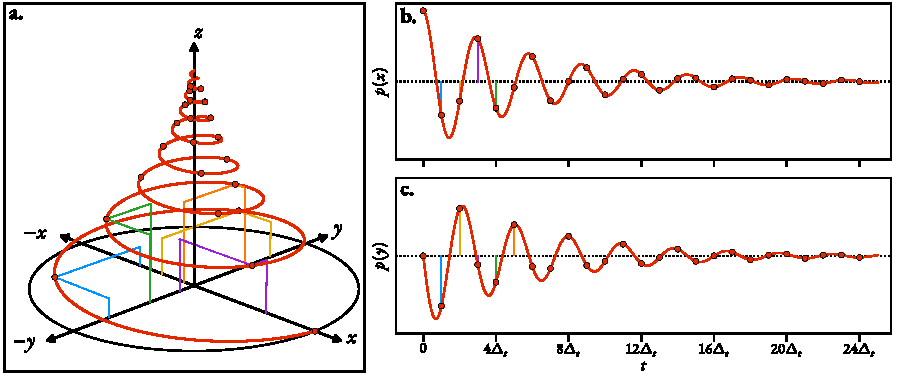
\includegraphics{quadrature_detection/quadrature_detection.pdf}
    \caption[
        An illustration of the free evolution of the bulk
        magnetisation of an ensemble of spin-$\nicefrac{1}{2}$ nuclei
        according to the Bloch model.
    ]{
        \textbf{a.} An illustration of the free evolution of the bulk
        magnetisation of an ensemble of spin-$\nicefrac{1}{2}$ nuclei
        immediately after the application of a $\ang{90}_y$ pulse according to
        the Bloch model.
        The projections of the magnetisation vector onto the
        $x$- and  $y$-axes are plotted in panels \textbf{b.} and \textbf{c.},
        respectively. Modern \acs{NMR} spectrometers utilise quadrature
        detection, such that the $x$- and  $y$- projections of the time-varying
        magnetisation is sampled at regular intervals, separated by $\Dt$.
        The resulting \acs{FID} is given by the complex value $p(x) + \iu
        p(y)$.
    }\label{fig:quadrature}
\end{figure}

\subsection{The NMR Spectrometer}

Modern \ac{NMR} spectrometers are capable of conducting a plethora of
experiments to help gain insights into chemical systems of interest.
In essence, a spectrometer comprises a high-field magnet, a probe, components
which are used to transmit \ac{RF} pulses to the probe, and components which
are used to process the resulting signal from the probe. A brief summary of
these is now given.

\subsubsection{The Magnet}
The static $\symbf{B}_0$ field is generated by a magnet, composed of a
superconducting solenoid immersed in liquid helium. Common materials used for
the solenoid include Nb-Ti alloy and Nb\textsubscript{3}Sn. To minimise the
extent of helium evaporation, the dewar containing the helium is lined with
a thermal radiation shield. The helium dewar is then surrounded by a larger
dewar containing liquid nitrogen. A bore passes through the $z$-direction of
the magnet, which is maintained at a user-controlled temperature. Within the
bore sits the probe as well as the sample. Magnets with high field
strengths are desirable, as both the resolution ($\propto B_0$) and sensitivity ($\propto
B_0^{\nicefrac{3}{2}}$) of the data are affected. At the
time of writing, commercial spectrometers which operate at and above a
\proton\ Larmor frequency of \qty{1}{\giga\hertz} (\qty{23.5}{\tesla}) exist,
though these are uncommon and are employed primarily for the study of large
biomolecules. For most applications, including the study of small molecules,
spectrometers with more modest field strengths are typically adequate.

A field-frequency \emph{lock} is used to ensure the stability of the magnetic
field.  The lock is a small \ac{NMR} spectrometer, typically
tuned to \textsuperscript{2}H\footnote{
    \textsuperscript{2}H-enriched solvents are routinely used to make up
    \ac{NMR} samples. In \proton\ \ac{NMR} experiments, this ensures that an
    extremely intense signal due to the solvent does not dwarf the signals from
    other spins in the sample. This makes \textsuperscript{2}H a suitable
    nucleus to monitor by the lock, as it is ubiquitous, but rarely directly
    studied.
}, which monitors the sample \textsuperscript{2}H resonance frequency over
time. If the frequency begins to drift, implying that the field strength is
changing, the current in the ``$Z_0$ coil'' is adjusted to ensure the
\textsuperscript{2}H frequency is maintained.

To maintain high spatial field homogeneity (a necessity for data with
acceptable resolution) a series of coils called \textit{shims} surround the
sample. Each coil produces a weak magnetic field with a specific spatial
profile according to a spherical harmonic function, which can cancel out any
inhomogeneity inherent to the main magnet.

\subsubsection{The Probe}
The probe sits inside the bore of the magnet, and features the coil(s) used to
pulse the sample with \ac{RF} radiation. The same coil(s) also
receive the response from the sample. The principle source of noise in
\ac{NMR} experiments is thermal noise within the probe circuitry. For
this reason, cryogenic probes\cite{Kovacs2020} have become a popular
development, in which the transmit/receive coil(s) and other probe electronics
are maintained at a very low temperature (typically about $\num{20}
\si{\kelvin}$).

\subsubsection{The Transmitter}
The transmitter is responsible for the generation of \ac{RF} pulses
with specified power, timing and phase.
A synthesiser acts as an \ac{RF} source, producing a continuous carrier wave at
or very close to the Larmor frequency of the target nucleus. This frequency
($\omega_{\text{RF}}$) can be adjusted in order to determine the center of the
spectrum. The difference between the carrier frequency and the reference
``basic frequency'' of the spectrometer is referred to as the \emph{transmitter
offset} $\foff$.  The output of the synthesiser is gated to ensure pulses are
applied at the desired times. An attenuator and amplifier then adjust the power
of the pulse, which travels to the probe.

\subsubsection{The Receiver}
During acquisition, the time-varying current induced in the probe coil(s) by
the sample magnetisation is
sent to a receiver, which comprises a series of components which convert it
to the \ac{FID} which is stored in computer memory. One of the processes
that the receiver is responsible for is \emph{quadrature
detection}\cite[Section 13.6]{Keeler2010},
which enables two orthogonal transverse components of the magnetisation to
be detected, and is crucial to produce spectra which are frequency
discriminated (see Section \ref{subsec:mulitdim}).
This is achieved by splitting the signal into two channels. Both
signals, which are of very high frequency (\unit{\mega\hertz}) are mixed with
a reference signal of frequency $\omega_{\text{RF}}$, such that a low-frequency
signal (\unit{\kilo\hertz}) is generated, along with a very high frequency
signal. One of the reference signals possess a phase which is shifted by
\ang{90} relative to the other one, such that the two channels constitute a
quadrature pair. The signals are then sent through a low-pass filter to remove
the high frequency component produced through mixing. Finally, an analogue to
digital converter translates the signal to the real and imaginary components of
a binary dataset which is stored in memory.

\subsection{The structure of the \acs{FID}}
The result of running an \ac{NMR} experiment is an \ac{FID} $\by$ which is sampled at
equally-spaced time-points, separated by time $\Dt$:
\begin{equation}
    \begin{split}
        \by &= \begin{bmatrix}
            y_0 & y_1 & y_2 & \cdots & y_{N-1}
      \end{bmatrix}\T\\
      &\equiv
      \begin{bmatrix}
          y(t=0) & y(t=\Dt) & y(t=2\Dt) & \cdots & y(t=(N-1)\Dt)
      \end{bmatrix}\T
    \end{split}
\end{equation}
where $y(t)$ is the (continuous) variation of the generated signal with time,
and $N$ is the number of points sampled. The inverse of the sampling rate,
$\nicefrac{1}{\Dt}$ is the \emph{sweep width} $\fsw$ which
defines how wide the range of samplable frequencies is, in accordance with the
Nyquist theorem\cite{Shannon1949}.

\acp{FID} adopt the form of a summation of $M \in \mathbb{N}$ complex
exponentials (signals). Each signal will be subjected to damping due to
transverse relaxation, which is typically exponential in nature. An \ac{FID}
acquired with $N$ samples $\by \in \mathbb{C}^{N}$ therefore takes the form
\begin{subequations}
    \begin{gather}
        y_n = x_n(\bth) + w_n \quad
            \quad \forall n \in \lbrace 0, 1, \cdots, N - 1 \rbrace,
            \label{eq:y=x+w} \\
        x_n(\bth) =
        \sumM \amexpphim \exp\left(
            (2 \pi \iu (f_m - \foff)- \eta_m ) n \Dt
        \right).
        \label{eq:x}
    \end{gather}
    \label{eq:1d}%
\end{subequations}%
\eqref{eq:1d} indicates that \iac{FID} comprises contributions from the
(deterministic) evolution of the spin magnetisation $\bx$ and experimental
noise $\bw$ (\emph{vide infra}). Each signal which contributes to $\bx$ is
defined by four parameters:
\begin{itemize}[label={}]
    \item Amplitude $a \in \mathbb{R}_{>0}$ ,
    \item Phase $\phi \in (-\pi, \pi]$ (\unit{\radian}),
    \item Frequency $f \in \left[\hspace*{2pt}\foff - \nicefrac{1}{2} \hspace*{2pt}
        \fsw, \foff + \nicefrac{1}{2} \hspace*{2pt}\fsw \right]$ (\unit{\hertz}),
    \item Damping factor $\eta \in \mathbb{R}_{>0}$ (\unit{\per\second}).
\end{itemize}%
The influence the four parameters have on a signal is depicted in panels
a1--d1 in Figure \ref{fig:amp-phase-freq-damp}.
\Iac{FID} can therefore be parameterised by the vector $\bth \in
\mathbb{R}^{4M}$:
\begin{equation}
    \bth =
    \begin{bmatrix}
        \symbf{a}\T & \symbf{\phi}\T & \symbf{f}\T & \symbf{\eta}\T
    \end{bmatrix}\T,
\end{equation}
where $\bda \in \mathbb{R}^M = [a_1 \hspace{2pt} a_2 \hspace{2pt} \cdots
\hspace{2pt} a_M]^{\mathrm{T}}$ is a vector of all amplitudes, $\bdphi \in
\mathbb{R}^M$ is a vector of all phases, etc.

Multidimensional experiments involve incrementing one or more delay within the
pulse sequence, in order to obtain an array of \ac{1D} \acp{FID}. In a
$D$-dimensional dataset, each contributing signal is parameterised by an
amplitude and phase as before, along with $D$ distinct frequencies and damping
factors, such that a general parameter vector  $\bth \in \mathbb{R}^{2(1+D)M}$
is given by
\begin{equation}
    \bth =
    \begin{bmatrix}
    \symbf{a}\T &
    \symbf{\phi}\T &
    {\bdfone}\T &
    \cdots &
    {\bdfD}\T &
    {\bdetaone}\T &
    \cdots &
    {\bdetaD}\T
    \end{bmatrix}\T,
    \label{eq:theta}
\end{equation}
where $\bdfD$ and $\bdetaD$ are the frequencies and damping factors in the
actively acquired (direct) dimension, and $\bdfone$ -- $\bdfDminusone$ and
$\bdetaone$ -- $\bdetaDminusone$ are those for the indirect dimension(s).
Indirect dimensions can exhibit different forms of evolution, depending on
the precise nature of the pulse sequence. Two common functional
forms exist\cite[Section 4.3.4]{Cavanagh2007}. Signals of the form $\cos(2 \pi
f t)$ and $\sin(2 \pi f t)$ modulate the amplitude of the direct
dimension signal across increments, while those of the form $\exp(2 \pi \iu f
t)$ or $\exp(-2 \pi \iu f t)$ modulate the phase.  Amplitude- or
phase-modulated signals are often acquired as pairs when possible, as this
ensures that spectra with desirable properties can be generated (\emph{vide
infra}). In general, a $D$-dimensional \ac{FID} $\bY \in \mathbb{C}^{\None
\times \cdots \times \ND}$ can be expressed as
\begin{subequations}
    \begin{gather}
        \YnonenD = X_{\nonedotsnD}(\bth) + W_{\nonedotsnD},\\
        X_{\nonedotsnD}
            = \sumM \amexpphim \prodD
            \zeta^{(d)}\left(2 \pi \left(f^{(d)}_m  - \foffd\right) \nd \Dtd\right)
            \exp\left(-\eta^{(d)}_m \nd \Dtd\right),\\
        \zeta^{(d)}(\cdot)
        \begin{cases}
            = \exp(\iu\cdot) & d = D \\
            \in \left\lbrace \cos(\cdot), \sin(\cdot), \exp(\iu\cdot) \exp(-\iu\cdot)\right\rbrace & \text{otherwise}
        \end{cases},
    \end{gather}
    \label{eq:general-fid}%
\end{subequations}%
It is typical to assume that $\symbf{W}$ is an array of \ac{AWGN}, i.e.
the noise instances are described by a complex normal distribution with mean 0,
and pairs of noise instances are statistically independent, regardless of their
time separation:
\begin{equation}
    \begin{gathered}
        W_{\nonedotsnD} \coloneq w \sim
        \mathcal{N_C}\left(0, 2\sigma^2\right) \\
        \implies \Re\left(w\right) \upmodels \Im\left(w\right),
             \Re\left(w\right) \sim \mathcal{N}\left(0, \sigma^2\right),
             \Im\left(w\right) \sim \mathcal{N}\left(0, \sigma^2\right). \\
    \end{gathered}
\end{equation}
The extent by which a signal is corrupted by noise is given by the \ac{SNR},
the ratio of signal power and noise power:
\begin{equation}
    \SNR\left(\bY\right) \coloneq
        \frac{1}{2 \mathfrak{N} \sigma^2}
        \sum_{\none=0}^{\None-1} \cdots \sum_{\nd=0}^{\ND-1}
        \left \lvert X_{\nonedotsnD} \right \rvert^2,
\end{equation}
where $\mathfrak{N} \coloneq \None \cdots \ND$ is the total number of points
the signal comprises. Due to the large dynamic range of the \ac{SNR} across
datasets, it is common to express it using a logarithmic scale instead,
in units of decibels (\unit{\deci\bel}):
\begin{equation}
    \begin{split}
        \SNR_{\unit{\deci\bel}} &\coloneq 10 \log_{10} \left(\SNR\right).
    \end{split}
\end{equation}
